\section{本轮概率对照与最小 Codex 实验协议}

\subsection{新增完成：真实二单元的带噪后验积分}

在前述冻结二单元合同上，取材料域 $[0.5,4]^2$、正规化先验
\begin{equation}
\rho(x_1,x_2)=x_1/27.5625,
\end{equation}
中心数据 $y=\F(1,3)$。这是一个明确采用有限噪声 likelihood 的观测实例；无需随机加入一份噪声才能定义后验。四个复通道实化为八个独立噪声分量，每个实部/虚部的标准差为 $\sigma=0.001$：
\begin{equation}
L(x)=\exp\{-\norm{\F(x)-y}_F^2/(2\sigma^2)\}.
\end{equation}
该约定对应复噪声方差 $\E|\eta_{rs}|^2=2\sigma^2$，与其他实验的 complex variance 定义不混用。

原材料矩形域用直接解析 $2\times2$ current 公式积分，quotient 用独立的对称有理公式与有序根三角域参数化积分。非光滑事件 $x_1>x_2$ 在其三角域内单独积分。每种方法均使用 32、64 阶 Gauss--Legendre 收敛对照；另用五个材料点的数值矩阵求解检查两个解析响应公式。

\begin{longtable}{@{}p{.28\textwidth}p{.22\textwidth}p{.22\textwidth}p{.19\textwidth}@{}}
\toprule 任务 & 原材料积分 & 正确商积分 & 均匀分支错误对照\\\midrule\endhead
缩放证据 $Z=\int\rho L$ & $0.1595738663$ & $0.1595738663$ & 相同\\
$\E[x_1\mid y]$ & $2.3865979378$ & $2.3865979378$ & $2.0542167027$\\
$\E[x_2\mid y]$ & $1.7218354676$ & $1.7218354676$ & $2.0542167027$\\
$\Pr(x_1>x_2\mid y)$ & $0.6751644709$ & $0.6751644709$ & $0.5$\\
$\E[x_1^2\mid y]$ & $6.2541540016$ & $6.2541540016$ & $4.9149818080$\\\bottomrule
\end{longtable}

错误对照\textbf{保留了完全相同的 quotient posterior 与证据}，只把条件分支权重改成 $1/2,1/2$。所以这不是拟合不够好的模型；它直接证明正确可观测世界仍不足以保证正确材料世界。

32 到 64 阶的最大证据相对差约 $2.19\times10^{-9}$，最大任务差约 $1.21\times10^{-8}$；两种 64 阶协议的差约为 $10^{-15}$。这是数值收敛和独立参数化的交叉验证，没有严格区间积分误差证书。

总费用为 15,360 次完整解析 likelihood 计算，其中原 current 解析响应 10,245 次、quotient 有理响应 5,125 次（含响应独立校验）；另有五次 $2\times2$ 数值分解、十个复 RHS。微小模型的毫秒级时间不用于宣称一般方法加速。此轮只完成已知 $C_2$ 结构的几何与概率阳性对照，尚未建立非对称分支发现、全材料图册或 Full66 后验结果。

\begin{figure}[p]
\centering
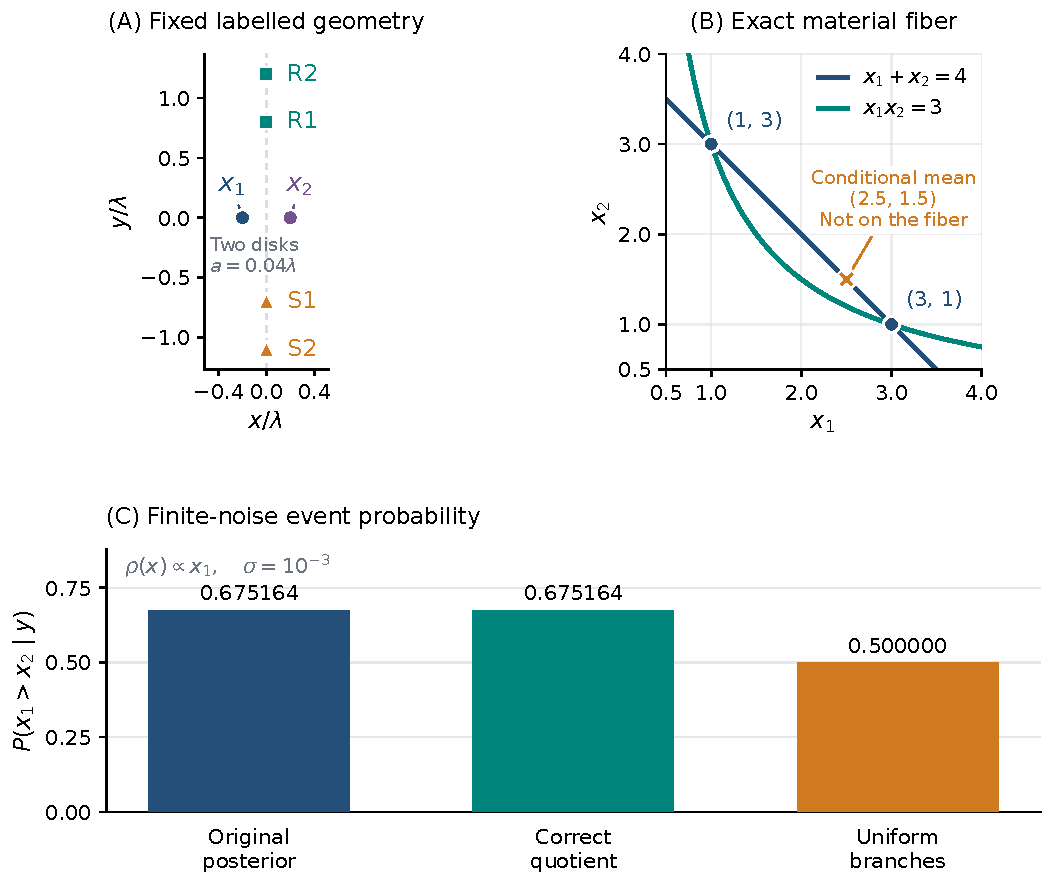
\includegraphics[width=\textwidth]{figures/two_cell_structure.pdf}
\caption{二单元 Maxwell 材料对称、可观测商与条件概率。（A）固定带标签的源、接收器及两圆盘材料几何。（B）$(1,3)$ 的精确材料纤维为 $x_1+x_2=4$ 与 $x_1x_2=3$ 的两个交点；在 $\rho\propto x_1$ 下，两支权重为 $1/4,3/4$，条件均值 $(2.5,1.5)$ 本身不在纤维上。（C）有限噪声下，原材料积分和正确商积分给出相同事件概率，均匀分支控制错误。面板 B 的精确纤维条件概率与面板 C 的带噪 posterior 是两个不同对象。}
\end{figure}
\clearpage

\subsection{输入、输出与独立合同}

附带的 \texttt{CODEX\_PROTOCOL\_ZH.txt} 是可直接交给 Codex 的完整执行协议。本节给出研究判断所需的紧凑版本。所有新实验在独立目录运行，R6/R7 的冻结报告、代码与账本只读。输入应包括：物理合同、原 prior、每个 decoder 的支持、源接收标签、Green 自项、噪声实化、任务定义、比较基线、种子与预算。

必须保存三类互不替代的证据：
\begin{enumerate}
\item \textbf{物理证据}：材料、全源电流、完整复预测、构成残差、被动性、prior 支持、resolvent 稳定性和独立复核。
\item \textbf{代数几何证据}：生成元恒等式/逆/组合、适用域、数值秩全谱、分支代表、连续参数、chart 转移、判别式事件及覆盖级别。
\item \textbf{概率与成本证据}：原测度、分支权重、coarea/恢复 Jacobian、参考积分、遗漏资格、失败尝试、全部分解与 RHS、CPU/wall time、内存。
\end{enumerate}

\subsection{E0--E4 的依赖顺序与成功门}

\begin{longtable}{p{.10\textwidth}p{.37\textwidth}p{.43\textwidth}}
\toprule 阶段 & 最小输入与测试 & 成功门与停止条件\\\midrule\endhead
E0 & $z^n$、圆、$a+b^2$、$V=QD$、三次映射、有限噪声链；明确 prior。 & 解析逆像、轨道、组合及概率对照均正确。错把 gauge 当材料或错权重时先停止修复。\\
E1 & 已完成两 cell 阳性；再用非对称 4--9 cell 真实 Green 模型。 & 完整物理验证；至少一个暗电流不可实现反例；扩展研究需真实不同材料或独立正则纤维依据。\\
E2 & 同一批材料及同一 prior；完整 Fourier/Wavelet、合法 Gaussian、材料 tangent、current chart。 & 往返材料保持，先验推前一致，支持变化单独标记。仅换基不算发现物理多解。\\
E3 & 从 E1 已有独立歧义证据的系统出发；比较 Full-J、multi-start、continuation、适用 CSI/SOM。 & 精确生成元须证闭合/逆/合法域；更强覆盖需限定域证书。只有端点或靠放松容差则降级。\\
E4 & 低维可信原空间积分；正确纤维、均匀轨道与错误边缘对照。 & 证据、均值、非线性任务、事件、branch mass 全部匹配；否则只能称几何枚举。\\\bottomrule
\end{longtable}

\textbf{推荐下一项最小问题}：一个非对称 4--9 cell TM 系统，预先固定全部标签，选择合法实材料内点和明确的新 prior。先构造 $n>k$ 的小型子问题，以常秩与 $n-r>0$ 作为精确局部纤维存在的独立依据；再比较共享材料 current chart 与直接材料隐函数/Full-J chart 对同一连通纤维的合法覆盖和条件积分费用。这里的目标不是发现维数计数已保证的 null，而是检验图册是否\emph{更可计算}。

另设 $n\le k$ 或满列秩子问题寻找远处分支，允许结果为没有发现。不要在看到结果后删 receiver 来制造成功；如需不同采集，建立新 contract ID。原 Full66 的离散远分支问题与新完整材料的连续纤维问题应分别注册。

\subsection{预算、数值资格与比较阈值}

以下是后续\emph{建议预算}，不是本轮已经使用的费用：每 run 最多 10,000 个实际复线性 RHS、2 CPU 小时、8 GB 峰值内存；整轮 30,000 RHS 硬上限。CPU 按线程累计，wall time 另记。结构构建、失败路径与认证都计入，不通过另开 run 绕过总上限。

float64 初筛可预注册归一化状态残差与完整观测差均不超过 $10^{-10}$，但这只是浮点门槛。数学精确只来自恒等式、符号推导或严格区间证书。数值 rank 记录缩放、全部谱、阈值与独立导数检查；不得把 $10^{-8}$ 以下的值直接当作零。

有限噪声验收始终对同一个 $y$，使用声明的 covariance 和 likelihood；噪声球可按预定 Gaussian 分位数选定，但仍不是等价类。路径相邻距离不能替代锚点检查。

E4 参考证据宜达到 $10^{-6}$ 或更好的数值精度；两种正确算法的证据相对差不超过 $\max(10^{-4},10\times\text{参考误差})$，归一化材料均值误差不超过 $10^{-4}$，事件/分支概率误差不超过 $10^{-3}$。Monte Carlo 则用预注册置信区间和 ESS。参考不够准时结论是参考不足，不事后放宽门槛。

效率门可预注册为相同覆盖与任务误差下总成本改善至少 $20\%$，并报告全部重复结果；这只是首轮决策阈值，不是统计显著性定理。小系统时间若由解释器或内存开销主导，不应外推为 Maxwell 大规模加速。

\subsection{后续三种决策}

\textbf{STOP}：只有非法暗电流；跨表示只是重复材料；exact 声明依赖放宽容差；原 prior 被换掉；缺乏比普通 corrector/continuation 更好的覆盖或费用；或者预算到限。停止对应研究主张，保留所有负面证据。

\textbf{CONDITIONAL GO}：有合法的非对称材料纤维/分支，或有独立覆盖证书，但正确概率或费用收益仍缺一项。下一轮只解决明确缺口。

\textbf{GO}：非对称小型 Maxwell 中获得可核验的更好分支覆盖、可计算图册或净物理费用收益，E4 正确测度通过，并与最强适用基线比较成立。之后才设计 Full66 或完整 576 实材料实验，二者继续分开。

\section{七个命题的答案与论文原创性判断}

\subsection{七个问题的条件答案}

\begin{longtable}{p{.08\textwidth}p{.25\textwidth}p{.57\textwidth}}
\toprule 命题 & 结论 & 关键条件或反例\\\midrule\endhead
1 & 简单群只在额外结构下完整刻画纤维。 & 集合层总有巨大置换群；光滑作用需等秩、等响应像，完整轨道需齐性/主丛等结构。三次实映射与自交浸入反例否定通用简单群。\\
2 & 跨 decoder 图册应先除 gauge，关系 decoder 用关联状态。 & submersion 可取局部 section；不同维数可同材料，非单射过渡一般不可逆。严格保材料循环不产生新世界。\\
3 & 常秩局部纤维维数为 $d-r$，满列秩局部单射。 & 不排除远处离散逆解。两 cell Maxwell 同时有 rank 2 与两个分支；Full66 rank66 不支持局部连续群。\\
4 & 有限噪声邻接不传递，也不构成等价群。 & 固定锚点、likelihood、log-ratio/TV 界与遗漏质量分开处理；近邻连通分量不是物理纤维。\\
5 & 可只反演商并复用 prior 核，当且仅当 likelihood 因子化。 & 标准 Borel disintegration；Gaussian 全数据族对应 forward 因子化；单点 quotient 不能替代带噪 quotient posterior。\\
6 & 有限固定生成元不能逐点列举连续纤维。 & 连续流族在同一正则连通分量上有条件覆盖；其他分量/strata 需额外箭头与证书；monodromy 需有限覆盖。\\
7 & 成本收益有条件，不能由代数名称保证。 & 已知对称可复用预测；current lift 可能膨胀，精确轨道质量可含 permanent；要比较冷启动总成本与任务误差。\\\bottomrule
\end{longtable}

\subsection{哪些内容已经属于成熟数学或既有电磁方法}

关系群胚、常秩/轨道定理、紧群不变量、覆盖 monodromy、disintegration/coarea、MH、Rao--Blackwell、LIS 以及数值代数几何都不能作为本研究独立首创。Maxwell 非辐射源、转换光学张量等价和 CSI/SOM 状态 lifting 也已有对应研究。

特别值得警惕的是两条重叠：一是把 Maxwell 离散状态写成多项式并用 homotopy 找根，并非新的研究概念；Everett 1996 已在小 Helmholtz 逆问题中实际枚举正实根，Vasco 2000 进一步研究代数化和消元。[R12,R13] 二是 current 的确定/模糊分解和材料显式更新已有 CSI/TSOM 前例。[R10,R11] 本轮二单元推导适合作为可审计的验证基准，尚不足以构成强 TAP 的核心贡献。

\textbf{近期直接先例。} Everett 于 2026-10-09 在线发表的研究，已对一维/二维电磁扩散的离散材料多项式系统，使用周期辅助参数和 Euler--Newton 路径寻找同数据的多个根，并区分正、负电导率候选。[R22] 因而 ``电磁逆问题多项式化后从一个解追踪其他解'' 也不能作为 Z-ALG 首创。

对这类方法的数学解释仍须独立审核：根集不自动成为循环群；往返线段在唯一正则提升下没有非平凡 monodromy，前文已经给出证明及奇异例外。$N$ 个方程、$N$ 个未知量也不意味着至多 $N$ 个根，反例 $x_i^2-1=0$ 有 $2^N$ 个非奇异根；一般零维多项式系统需采用正确的次数或稀疏根数界。新论文提供的有价值候选发现应与这些未成立的一般推断区分。

后续 E3 的普通 continuation 基线应包含适用于同一问题的此类周期参数跟踪，并保存奇异事件和跳支。不能因为路径法有合格端点就赋予它全覆盖、物理可行路径或 posterior 权重；同样不能因为其全局解释不足便忽略其实际搜索价值。

\subsection{最有希望的论文贡献：依次排序}

\textbf{第一优先：材料一致性与可认证纤维图册。} 在真实、非对称、多源 Maxwell 子问题中，把接收器暗空间缩为可实现材料图册；给出节点、被动性、prior 支持和 resolvent 的完整处理，并在有界材料域上证明或严格认证比基线更多的分支/分量。独立价值来自材料覆盖，不来自联立方程本身。

\textbf{第二优先：正确概率的可计算分支/纤维积分。} 在相同原 prior 下实现条件核、图册去重和任务积分，证明误差或遗漏界，并以相同费用展示对材料事件和风险的改善。这里的创新应是 Maxwell 特有的可计算分解或证书，而非重新证明通用 Bayes 分解。

\textbf{第三优先：新的合法材料变换或实验设计结论。} 若能在普通标量、固定磁导率的合理采集下发现非显然的精确变换，给出明确条件、覆盖和费用，可能构成独立理论论文。现有两 cell 镜像交换太简单，只能作为阳性例子；全各向异性坐标变换则已有文献，不宜包装成新结论。

\textbf{第四优先：有条件的 quotient imaging 加速。} 必须表明 quotient prior、likelihood 和条件生成器整体比直接反演便宜，且任务误差/覆盖相同。若只是把 $F(m)$ 命名为 $u$，然后在每个 $u$ 重新求一次原逆问题，则没有算法贡献。

\subsection{对强 IEEE TAP 的现实判断}

以目前结果直接写成 ``群胚统一 Maxwell 多解''，发表价值不足；抽象统一与几个 toy 不会消除与既有理论的重叠。以目前结果组织一份严谨研究设计和可复现实验基准，则是有价值的起点。

若后续取得非对称、多源物理模型上的新覆盖证书、材料有效的低费用生成器，或正确概率积分的任务收益，并展示适度网格/多频验证及离散误差影响，可以形成独立 Maxwell 方法论文。若主体贡献更偏代数复杂性、奇异测度或一般分层定理，数学反问题或计算数学期刊也可能更匹配；不能用 TAP 标签替代实际电磁增量。

本轮建议为\textbf{CONDITIONAL GO：建立 Research Z-ALG，但先以材料约束和正确测度为主线}。最小下一问题已经明确：在一个非对称小型 TM 系统的已知正维正则纤维上，比较 current 图册与直接材料 continuation 的合法覆盖、条件积分和总成本。若这一关没有优势，应停止扩大 ``通用代数探索''；若成功，再分别研究离散远分支和原 Full66 适用性。

用户提出的愿景在数学上可实现的精确形式是
\begin{equation}
y\longmapsto\nu^y(du),\qquad
(u,\xi)\longmapsto M\sim K(\cdot\mid u),
\end{equation}
其中 $\xi$ 包含分支和连续纤维随机性，$K$ 严格来源于原材料 prior。最大的开放问题并不是这个分解是否存在，而是\textbf{能否对具体 Maxwell 合同把它构造得比直接后验计算更完整、更稳定或更便宜}。
